\subsection{Abstraction}

{ % all template changes are local to this group.
  \setbeamertemplate{navigation symbols}{}
  \begin{frame}[plain]
    \begin{tikzpicture}[remember picture,overlay]
      \node[at=(current page.center)] {
        
\includegraphics[width=\paperwidth]{degoes.png}
      };
    \end{tikzpicture}
  \end{frame}
}

{ % all template changes are local to this group.
  \setbeamertemplate{navigation symbols}{}
  \begin{frame}[plain]
    \begin{tikzpicture}[remember picture,overlay]
      \node[at=(current page.center)] {
        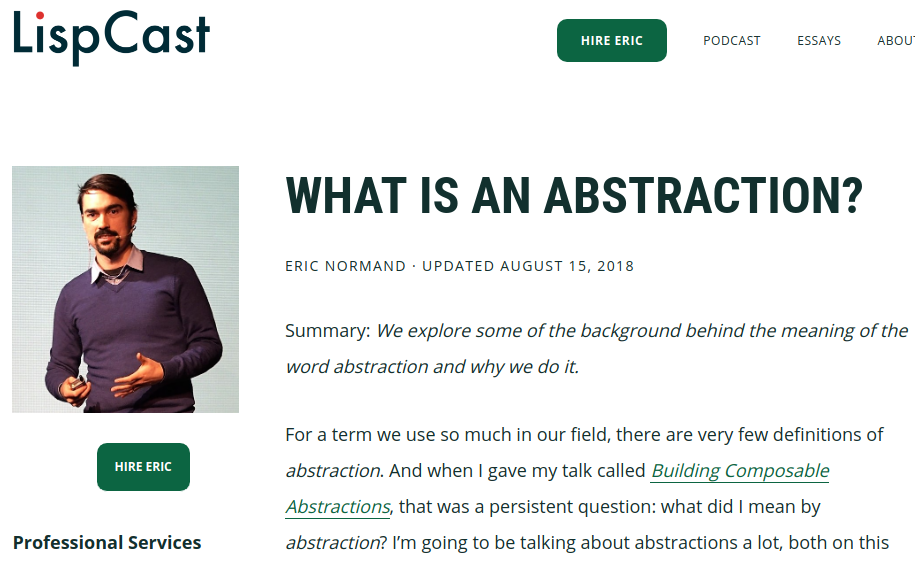
\includegraphics[width=\paperwidth]{normand-abst.png}
      };
    \end{tikzpicture}
  \end{frame}
}

{ % all template changes are local to this group.
  \setbeamertemplate{navigation symbols}{}
  \begin{frame}[plain]
    \begin{tikzpicture}[remember picture,overlay]
      \node[at=(current page.center)] {
        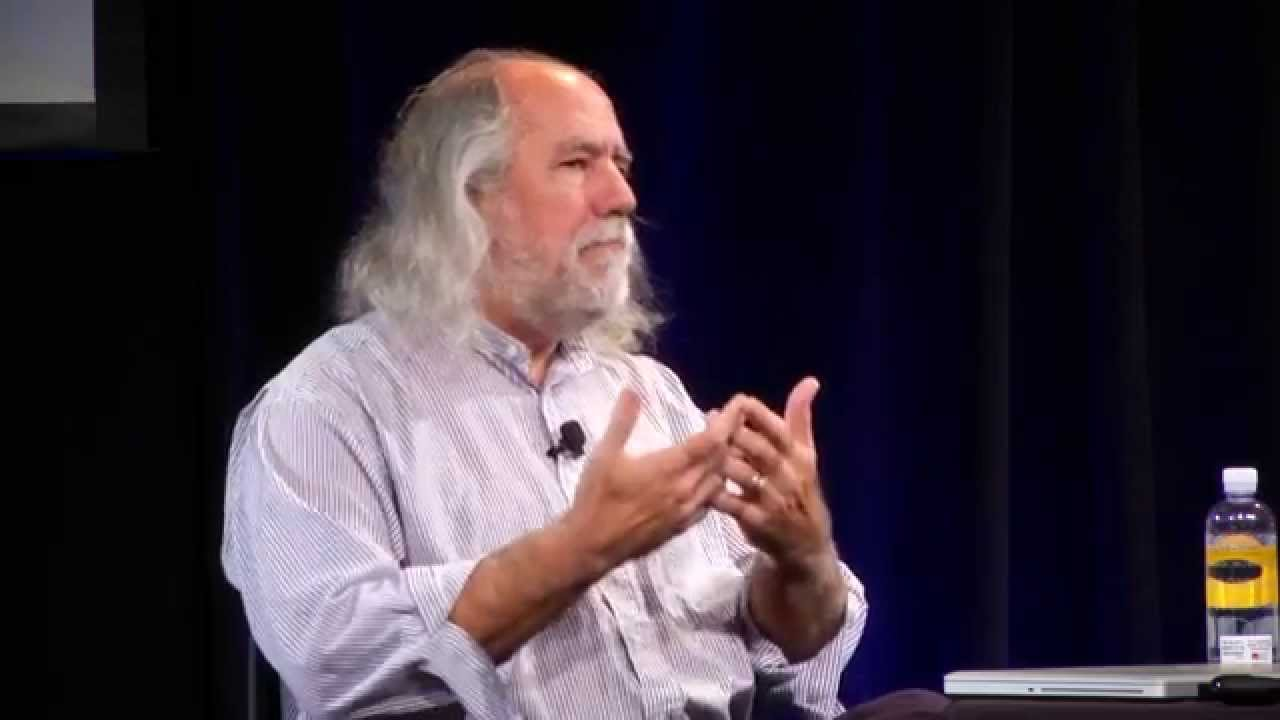
\includegraphics[width=\paperwidth]{grady-booch-explaining.jpg}
      };
    \end{tikzpicture}
  \end{frame}
}

{ % all template changes are local to this group.
  \setbeamertemplate{navigation symbols}{}
  \begin{frame}[plain]
    \begin{tikzpicture}[remember picture,overlay]
      \node[at=(current page.center)] {
        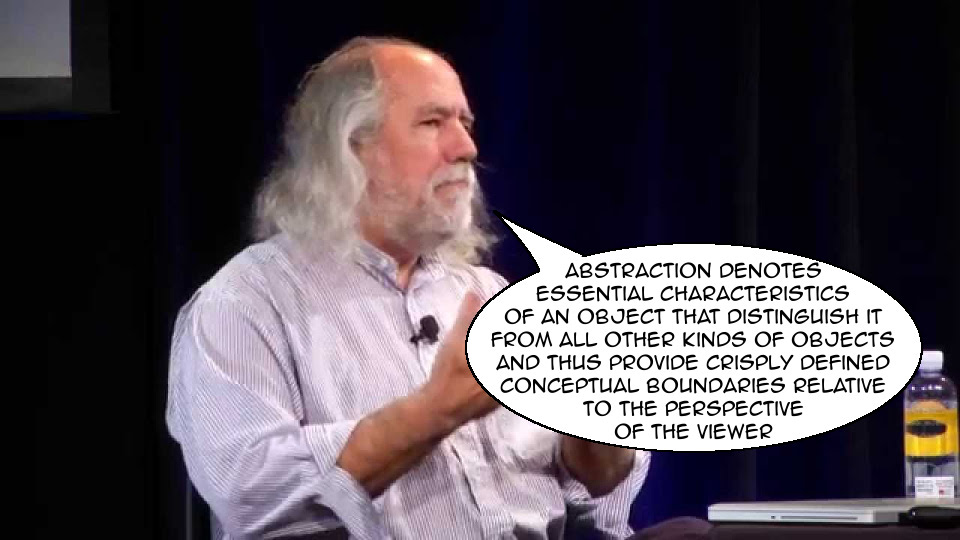
\includegraphics[width=\paperwidth]{grady-booch-abstraction.jpg}
      };
    \end{tikzpicture}
  \end{frame}
}

{ % all template changes are local to this group.
  \setbeamertemplate{navigation symbols}{}
  \begin{frame}[plain]
    \begin{tikzpicture}[remember picture,overlay]
      \node[at=(current page.center)] {
        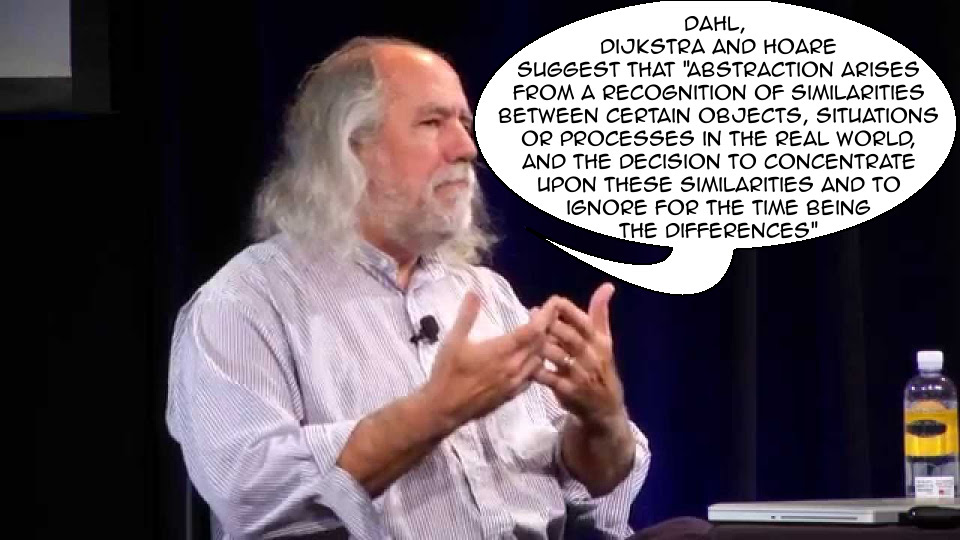
\includegraphics[width=\paperwidth]{grady-booch-dijkstra.jpg}
      };
    \end{tikzpicture}
  \end{frame}
}

{ % all template changes are local to this group.
  \setbeamertemplate{navigation symbols}{}
  \begin{frame}[plain]
    \begin{tikzpicture}[remember picture,overlay]
      \node[at=(current page.center)] {
        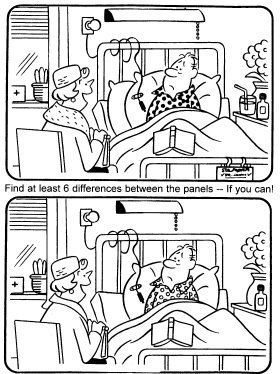
\includegraphics[width=0.3\paperwidth]{diff.jpeg}
      };
    \end{tikzpicture}
  \end{frame}
}

{ % all template changes are local to this group.
  \setbeamertemplate{navigation symbols}{}
  \begin{frame}[plain]
    \begin{tikzpicture}[remember picture,overlay]
      \node[at=(current page.center)] {
        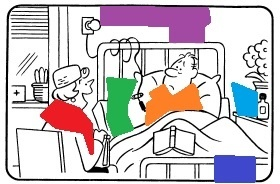
\includegraphics[width=0.3\paperwidth]{abstract.jpeg}
      };
    \end{tikzpicture}
  \end{frame}
}

{ % all template changes are local to this group.
  \setbeamertemplate{navigation symbols}{}
  \begin{frame}[plain]
    \begin{tikzpicture}[remember picture,overlay]
      \node[at=(current page.center)] {
        
\includegraphics[width=0.8\paperwidth]{abstract-holes.jpeg}
      };
    \end{tikzpicture}
  \end{frame}
}

\begin{frame}{Definition of abstraction I}
  \begin{description}
  \item [abstraction] the process of intentionally
    omitting (leaving out) certain detail in some mental representation
  \end{description}
\end{frame}

\begin{frame}{Definition of abstraction II}
  \begin{description}
  \item [abstraction] a mental representation which
    contains \textit{holes} that can be filled with some
    content (concretized)
  \end{description}
\end{frame}
